\documentclass[a4paper,10pt]{article}
\usepackage[utf8]{inputenc}
\usepackage[brazil]{babel}
\usepackage{listings}
\usepackage{enumerate}
\usepackage{graphicx}


\begin{document}
\lstset{language=c,numbers=left,numberstyle=\tiny,breaklines=true,frame=single}

\begin{titlepage}

\begin{center}
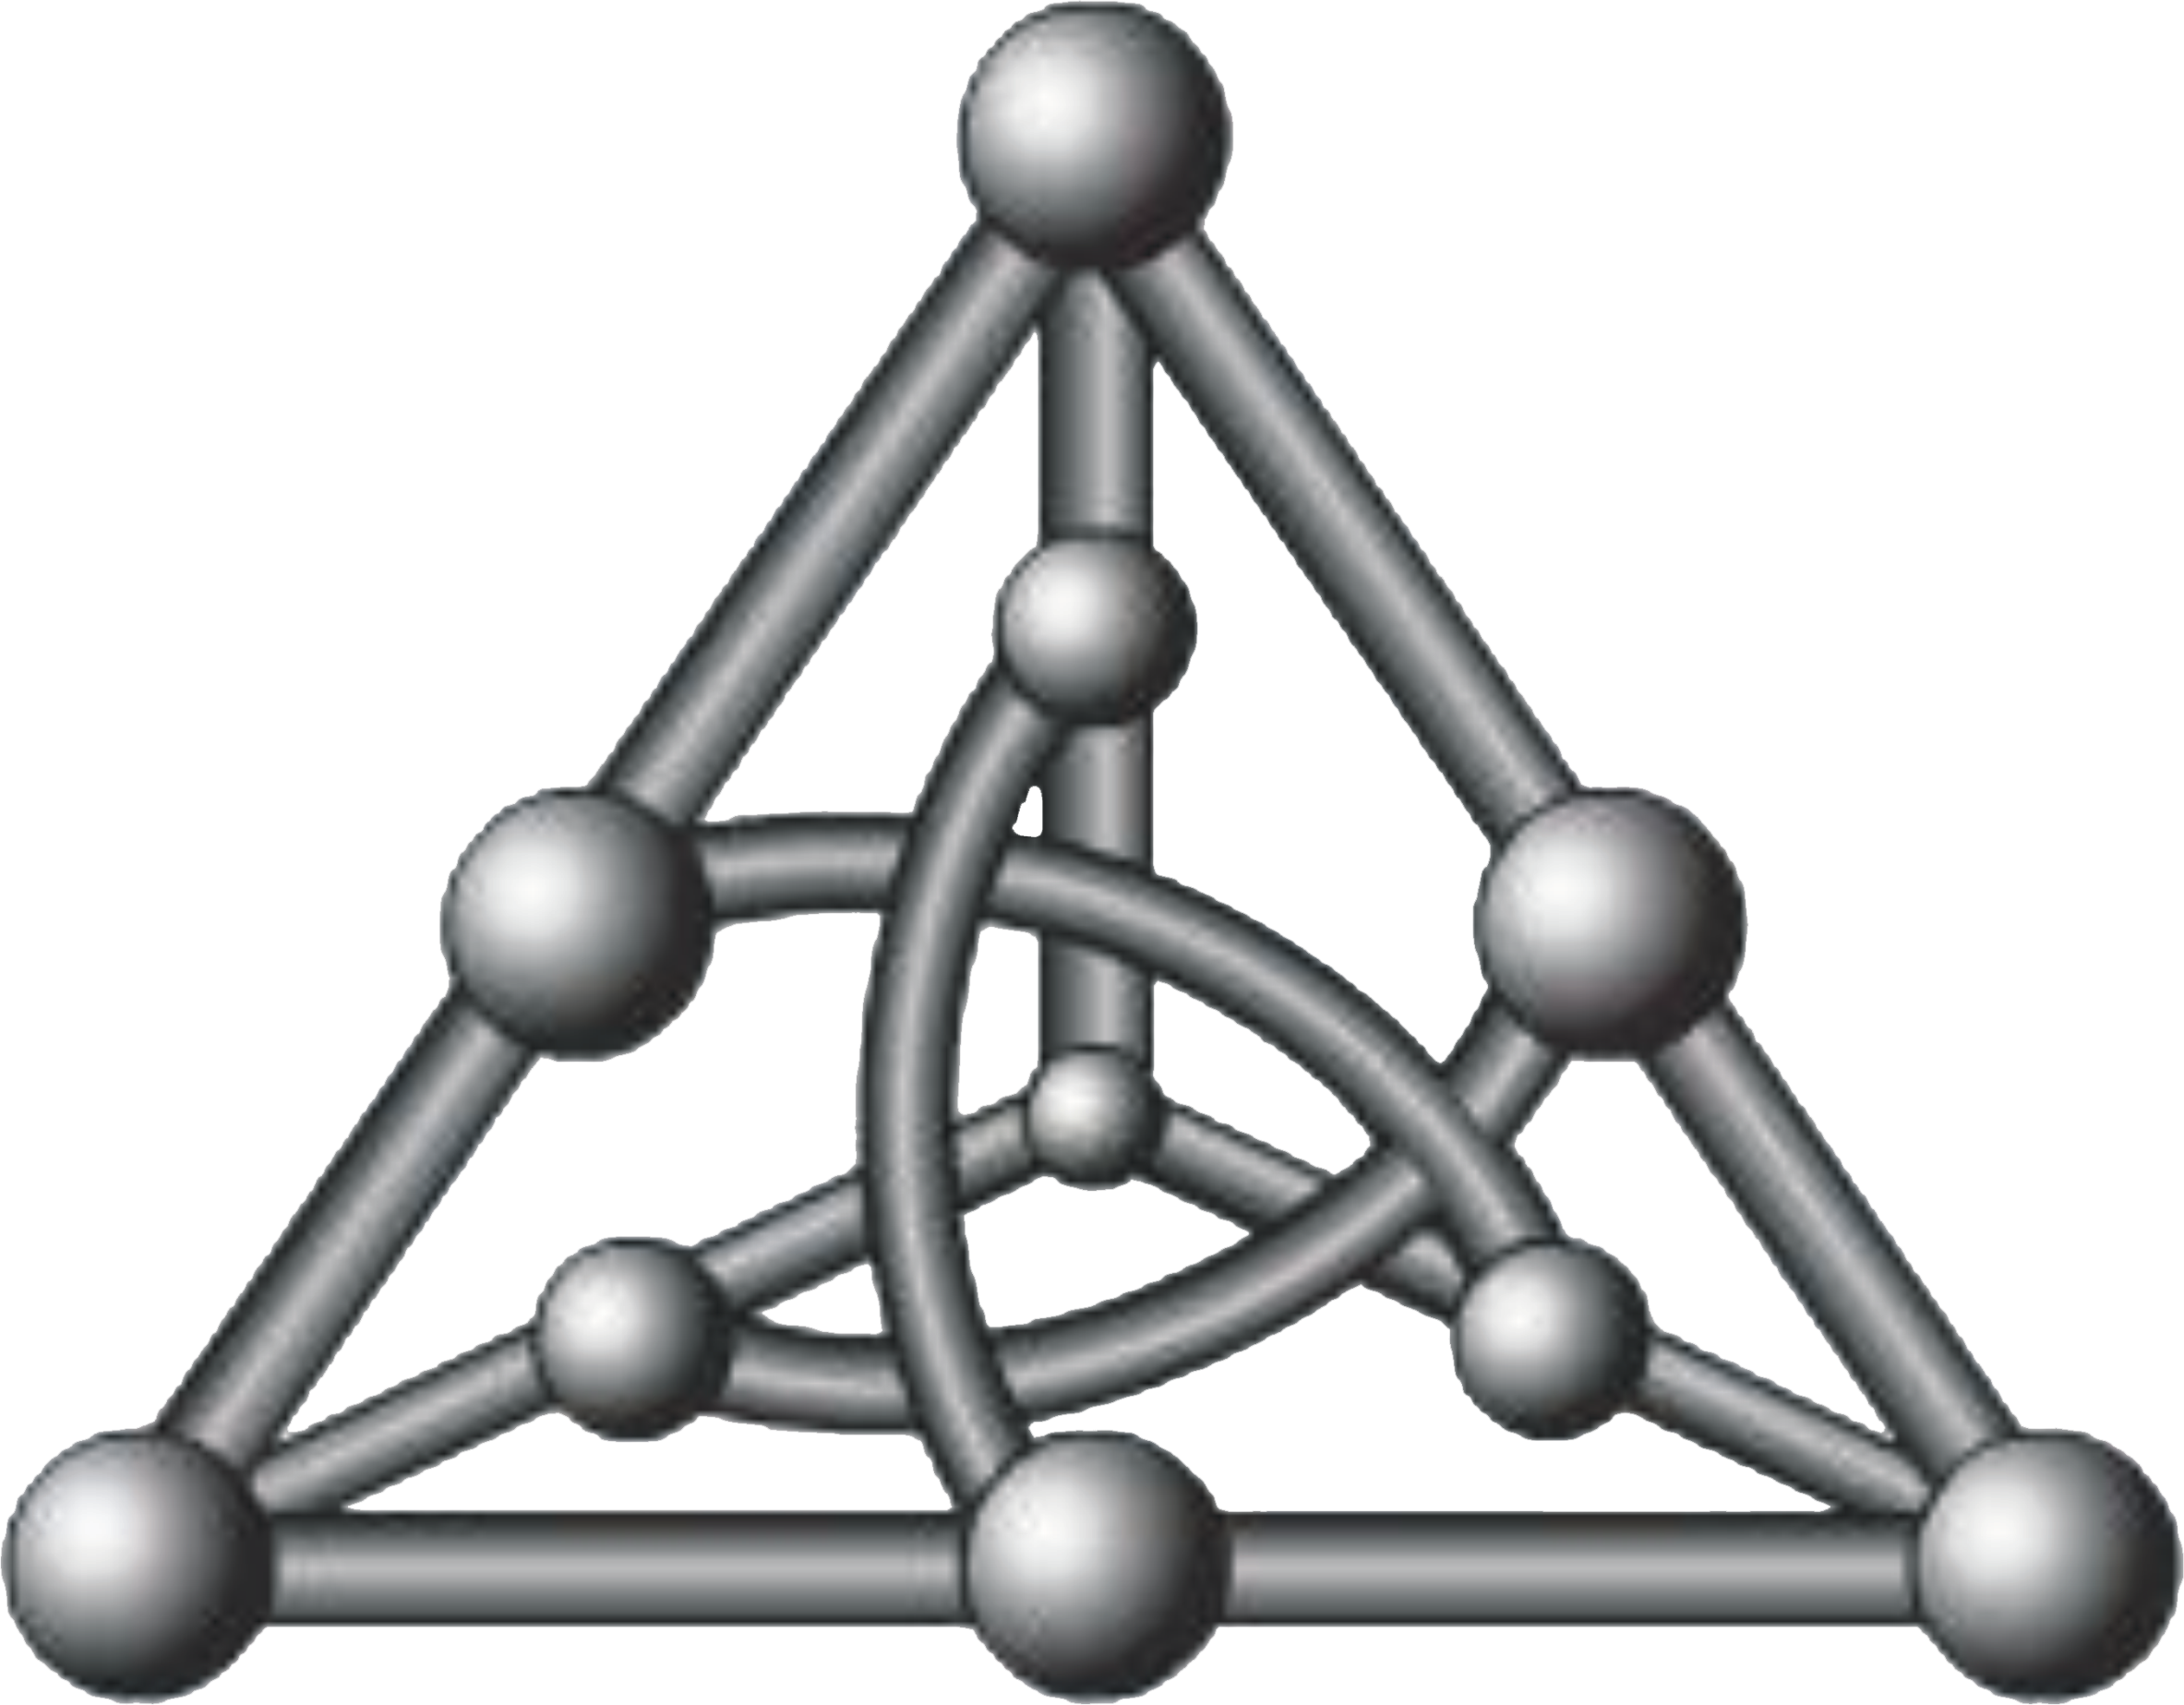
\includegraphics[width=2.5cm]{facom_t}\\[0.5cm]
\textsc{UFMS - Faculdade de Computação}\\[0.25cm]
\textsc{\LARGE Algoritimos de Programação II Turma 3}\\[0.5cm]
\textsc{Professor: Marco Aurélio Stefanes}\\[2.5cm]
{ \huge \bfseries Lista 01 \\[0.4cm] }
\end{center}
\vspace{10cm}


\begin{minipage}{1.6\textwidth}
\begin{center}
\emph{Aluno:} \\
Augusto Cesar de Aquino Ribas\\
Análise de Sistemas\\
\end{center}
\end{minipage}%

\end{titlepage}

\newpage
\section{Aula 01-03 : Exercícios. 1.5 a 1.9}

\begin{enumerate}

\item 
\begin{enumerate}[(a)]

\item Escreva uma função recursiva com a seguinte interface:\\

\begin{lstlisting}
int soma_digitos(int n)
\end{lstlisting}

que receba um número inteiro positivo $n$ e devolva a soma de seus dígitos.\\

\begin{lstlisting}
int soma_digitos(int n) {
  int soma;

  if((n/10)==0) {
    soma=n;
  } else {
    soma=n%10+soma_digitosR(n/10);
  }

  return soma;

}
\end{lstlisting}

\item Escreva um programa que receba um número inteiro $n$ 
e imprima a soma de seus dígitos. Use a função do item (a).\\

\begin{lstlisting}
#include <stdio.h>

int soma_digitos(int n) {
  int soma;
  if((n/10)==0) {
    soma=n;
  } else {
    soma=n%10+soma_digitosR(n/10);
  }
  return soma;
}

int main(void)
{
  int n;
  scanf("%d",&n);
  printf("Funcao recursiva: Soma dos digitos e %d\n",soma_digitos(n));
  return 0;
}
\end{lstlisting}
\end{enumerate} %letras
\pagebreak

\item  A \textbf{seqüência de Fibonacci} é uma seqüência de números inteiros positivos dada pela seguinte fórmula:
  \[ 
  \left\{ \begin{array}{rcl}
    F_1 & = & 1 \\
    F_2 & = & 1 \\
    F_i & = & F_{i-1} + F_{i-2},\ \textnormal{para}\ i\geq 3 
  \end{array}
  \right. 
  \]

\begin{enumerate}[(a)]
\item Escreva uma função recursiva com a seguinte interface:

\begin{lstlisting}
int Fib(int i)
\end{lstlisting}

que receba um número inteiro positivo $i$ e devolva o $i$-ésimo termo da seqüência de Fibonacci, isto é, $F_i$. 

\begin{lstlisting}
int fib(int i){

  if(i==1) {
    return 1;
  } else {
    if(i==2) {
      return 1;
    } else {
      return fib(i-1)+fib(i-2);
    }
  }
}
\end{lstlisting}
  
\item Escreva um programa que receba um número inteiro $i \geq 1$ e imprima o termo $F_i$ da seqüência de Fibonacci. 
Use a função do item (a).

\begin{lstlisting}
#include <stdio.h>

int fib(int i){
  if(i==1) {
    return 1;
  } else {
    if(i==2) {
      return 1;
    } else {
      return fib(i-1)+fib(i-2);
    }
  }
}

int main(void)
{
  int i;
  scanf("%d",&i);
  printf("Resultado = %d\n",fib(i));
  return 0;
}
\end{lstlisting}

\end{enumerate}
\pagebreak

\item O \textbf{piso} de um número inteiro positivo $x$ é o único inteiro $i$ 
tal que $i \leq x < i + 1$. O piso de $x$ é denotado por $\lfloor x \rfloor$.   

Segue uma amostra de valores da função $\lfloor \log_2 n \rfloor$:

  \begin{center}
    \begin{tabular}{*{13}{r}}
      $n$ & 15 & 16 & 31 & 32 & 63 & 64 & 127 & 128 & 255 & 256 & 511
      & 512 \\ \cline{2-13}  
      $\lfloor \log_2 n \rfloor$ & 3 & 4 & 4 & 5 & 5 & 6 & 6 & 7 & 7 &
      8 & 8 & 9  
    \end{tabular}
  \end{center}

\begin{enumerate}[(a)]
\item Escreva uma função recursiva com a seguinte interface:

\begin{lstlisting}
int piso_log2(int n)
\end{lstlisting}

que receba um número inteiro positivo $n$ e devolva $\lfloor \log_2 n \rfloor$. 

\begin{lstlisting}
int piso_log2(int n){
  if(n/2==0) {
    return 0;
  } else {
    return 1+piso_log2(n/2);
  }

}
\end{lstlisting}

\item Escreva um programa que receba um número inteiro $n \geq 1$ e imprima $\lfloor \log_2 n \rfloor$. 
Use a função do item (a).

\begin{lstlisting}
#include <stdio.h>

int piso_log2(int n){
  if(n/2==0) {
    return 0;
  } else {
    return 1+piso_log2(n/2);
  }

}

int main(void)
{
  int n;

  scanf("%d",&n);
  printf("%d\n",piso_log2(n));
  return 0;
}
\end{lstlisting}



\end{enumerate}

\pagebreak

\item Considere o seguinte processo para gerar uma seqüência de números.
Comece com um inteiro $n$. Se $n$ é par, divida por $2$.
Se $n$ é ímpar, multiplique por $3$ e some $1$. 
Repita esse processo com o novo valor de $n$, terminando quando $n = 1$.
Por exemplo, a seqüência de números a seguir é gerada para $n = 22$:

  \[
  22 \hspace*{.5cm} 11 \hspace*{.5cm} 34 \hspace*{.5cm} 17 
  \hspace*{.5cm} 52 \hspace*{.5cm} 26 \hspace*{.5cm} 13 \hspace*{.5cm} 
  40 \hspace*{.5cm} 20 \hspace*{.5cm} 10 \hspace*{.5cm} 5
  \hspace*{.5cm} 16 \hspace*{.5cm} 8 \hspace*{.5cm} 4 \hspace*{.5cm} 2
  \hspace*{.5cm} 1   
  \]

É conjecturado que esse processo termina com $n = 1$ para todo inteiro $n > 0$.
Para uma entrada $n$, o \textbf{comprimento do ciclo de $n$} é o número de elementos gerados na seqüência.
No exemplo acima, o comprimento do ciclo de $22$ é $16$. 

\begin{enumerate}[(a)]
  \item Escreva uma função não-recursiva com a seguinte interface:

\begin{lstlisting}
int ciclo(int n)
\end{lstlisting}

que receba um número inteiro positivo $n$, mostre a seqüência gerada pelo processo descrito acima 
na saída e devolva o comprimento do ciclo de $n$. 

\begin{lstlisting}
int ciclo(int n){
  int ciclo=1;
  while(n!=1) {
    if(n%2==0) {
      printf("%d ",n/2);
      n=n/2;
    } else {
      printf("%d ",n*3+1);
      n=n*3+1;
    }
    ciclo++;
  }
  return ciclo;
}
\end{lstlisting}

\pagebreak

\item Escreva uma versão recursiva da função do item (a) com a seguinte interface: 

\begin{lstlisting}
int cicloR(int n)
\end{lstlisting}

que receba um número inteiro positivo $n$, mostre a seqüência gerada pelo processo descrito 
acima na saída e devolva o comprimento do ciclo de $n$.

\begin{lstlisting}
int cicloR(int n){
  if(n%2==0) {
    printf("%d ",n/2);
    n=n/2;
  } else {
    printf("%d ",n*3+1);
    n= n*3+1;
  }
  if(n==1) {
    return 2;
  } else {
    return 1+cicloR(n);
  }
}
\end{lstlisting}
\pagebreak

\item Escreva um programa que receba um número inteiro $n \geq 1$ e determine a seqüência gerada 
por esse processo e também o comprimento do ciclo de $n$. Use as funções em (a) e (b) para testar. 
\end{enumerate}

\begin{lstlisting}
#include <stdio.h>

int ciclo(int n){
  int ciclo=1;
  while(n!=1) {
    if(n%2==0) {
      printf("%d ",n/2);
      n=n/2;
    } else {
      printf("%d ",n*3+1);
      n=n*3+1;
    }
    ciclo++;
  }
  return ciclo;
}
int cicloR(int n){
  if(n%2==0) {
    printf("%d ",n/2);
    n=n/2;
  } else {
    printf("%d ",n*3+1);
    n= n*3+1;
  }
  if(n==1) {
    return 2;
  } else {
    return 1+cicloR(n);
  }
}

int main(void)
{
  int x, saida;
  scanf("%d",&x);
  saida=ciclo(x);
  printf("\niterativo %d\n",saida);
  saida=cicloR(x);
  printf("\nrecursivo %d\n",saida);
  return 0;
}
\end{lstlisting}
\pagebreak


\item Podemos calcular a potência $x^n$ de uma maneira mais eficiente.
Observe primeiro que se $n$ é uma potência de 2 então $x^n$ pode ser computada usando seqüências de quadrados.
Por exemplo, $x^4$ é o quadrado de $x^2$ e assim $x^4$ pode ser computado usando somente duas multiplicações 
ao invés de três. Esta técnica pode ser usada mesmo quando $n$ não é uma potência de 2, usando a seguinte fórmula:


\[    x^n = \left \{ \begin{array}{ll}
        1\:, & \textnormal{se $n = 0$,} \\
        (x^{n/2})^2\:, & \textnormal{se $n$ é par,} \\
        x \cdot x^{n-1}\:, & \textnormal{se $n$ é ímpar.}
      \end{array} \right. \]

  
  
  
  
  \begin{enumerate}[(a)]
  \item Escreva uma função com interface

\begin{lstlisting}
int potencia(int x, int n)
\end{lstlisting}

que receba dois números inteiros $x$ e $n$ e calcule e devolva $x^n$ usando a fórmula acima.

\begin{lstlisting}
int potencia(int x, int n) {
  int num;
  if(n==0) {
    /*Se n e zero*/
    return 1;
  } else {
    if( (n%2) == 0 ) {
    /*Se n e par*/
      num=potencia(x,n/2);
      return num*num;
    } else {
    /*Se n e impar*/
      return x * potencia(x,n-1);
    }
  }
}
\end{lstlisting}

\pagebreak

\item Escreva um programa que receba dois números inteiros $a$ e $b$ e imprima o valor de $a^b$.
  \end{enumerate}
  
\begin{lstlisting}
#include <stdio.h>

int potencia(int x, int n) {
  int num;
  if(n==0) {
    /*Se n e zero*/
    return 1;
  } else {
    if( (n%2) == 0 ) {
    /*Se n e par*/
      num=potencia(x,n/2);
      return num*num;
    } else {
    /*Se n e impar*/
      return x * potencia(x,n-1);
    }
  }
}

int main(void) {
  int num, pot;
  scanf("%d %d",&num, &pot);
  printf("Resposta: %d\n",potencia(num,pot));
  return 0;
}
\end{lstlisting}

\end{enumerate} %Números
\pagebreak



\newpage
\section{Aula 05: Exercícios 2.6 a 2.10}

\begin{enumerate}
 
 
\item É verdade que $2^{n+1} = O(2^n)$? E é verdade que $2^{2 \cdot n} = O(2^n)$?

Sim, a notação do O ou notação assintótica utilizada para analisar o comportamento assintótico de funções,
ou seja, como é o crescimento destas, apesar da diferenças no expoentes pelos quais 2 está sendo elevado em cada caso,
em ambos os casos a função cresce exponencialmente como potencia de 2 como visto na figura.

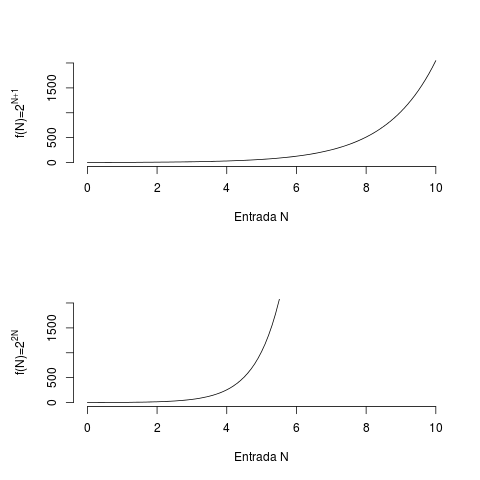
\includegraphics[width=10cm]{exercicio}\\

\pagebreak

\item Suponha que você tenha algoritmos com os cinco tempos de execução listados abaixo.
Quão mais lento cada um dos algoritmos fica quando você (i) duplica o tamanho da
entrada, ou (ii) incrementa em uma unidade o tamanho da entrada?

  \begin{enumerate}[(a)]
\item $n^2$\\
Nesse caso, se duplicamos o tamanho para $n^2$ teremos:\\
$(2\cdot n)^2$\\
$2^2 \cdot n^2$\\
$4 \cdot n^2$\\
Ou seja, ao dobrarmos o tamanho da entrada, quadruplicamos o tempo do algoritimo.\\
Para o casso de incrementarmos em uma unidade a entrada temos:\\
$(n+1)^2$\\
$(n+1) \cdot (n+1)$\\
$n^2+2 \cdot n+1^2$\\
$(2 \cdot n+1)+n^2$\\
Ou seja, se incrementarmos em uma unidade a entrada, aumentamos em $(2\cdot n+1)$ o tempo de execução do algoritimo.\\

\item $n^3$\\
Duplicando a entrada aumentamos em oito vezes o tempo de execução:\\
$(2 \cdot n)^3$\\
$(2^3) \cdot (n^3)$\\
$8 \cdot (n^3)$\\
Aumentando em uma unidade a entrada temos um aumento no tempo de execução 
em $3 \cdot (n + {1\over{2}} )^2 + {1\over{4}}$ unidades\\
$(n+1)^3$\\
$n^3+3n^2+3n+1$\\
$(3n^2+3n+1)+(n^3)$\\
$3 \cdot (n + {1\over{2}} )^2 + {1\over{4}}+(n^3)$\\

\item $100 \cdot n^2$\\
Duplicando a entrada aumentamos em quatrocentas vezes o tempo de execução:\\
$100 \cdot (2\cdot n)^2$\\
$100 \cdot 2^2 \cdot n^2$\\
$100 \cdot 4 \cdot n^2$\\
$400 \cdot n^2$\\

Aumentando em uma unidade a entrada temos um aumento no tempo de execução 
em$(200 \cdot n +100)$\\
$100 \cdot (n+1)^2$\\
$100 \cdot (n+1) \cdot (n+1)$\\
$100 \cdot (n^2+2 \cdot n+1^2)$\\
$100 \cdot n^2 + 200 \cdot n +100$\\
$(200 \cdot n +100) + 100 \cdot n^2$\\

\pagebreak

\item $n \cdot \log_2(n)$\\
Duplicando a entrada, dobramos o tempo de execução:\\
$2\cdot n \cdot \log_2(2\cdot n)$\\
$2\cdot n \cdot \log_2(2) \cdot \log_2(n)$\\
$2\cdot n \cdot 1 \cdot \log_2(n)$\\
$2\cdot n \cdot \log_2(n)$\\
$2\cdot (n \cdot \log_2(n))$\\

Aumentando em uma unidade a entrada temos um aumento no tempo de execução 
em bem pequeno, ja que ao dobrarmos o tamanho da entrada dobramos o tempo, 
então aumentar em uma unidade é relativamente pequeno\\
$(n+1) \cdot \log_2(n+1)$\\

\item $2^n$\\
Duplicando a entrada aumentamos em quadruplicamos o tempo de execução:\\
$2^{2 \cdot n}$\\
$(2^2)^n$\\
$4^n$\\

Aumentando em uma unidade a entrada, dobramos o tempo de execução\\
$2^{n+1}$\\
$2^n*2^1$\\
$2*2^n$\\


  \end{enumerate}

\item Suponha que você tenha algoritmos com os seis tempos de execução listados abaixo. 
Suponha que você tenha um computador capaz de executar 1010 operações por segundo
e você precisa computar um resultado em no máximo uma hora de computação. Para
cada um dos algoritmos, qual é o maior tamanho da entrada n para o qual você poderia
receber um resultado em uma hora?

Uma hora correponde a 60 minutos, como cada minuto tem 60 segundos, em uma hora temos 3600 segundos.
O computador pode realizar 1010 operações por segundo, logo podemos realizar no maximo 3636000 operações em uma hora.
Os valores de resposta são sempre o piso do valor calculado, já que não deve existir meia entrada.\\

Assim:

  \begin{enumerate}[(a)]
\item $n^2$\\
$n^2=3636000$\\
$n=\sqrt[2]{3636000}$\\
$n\approx{1906}$\\

\pagebreak

\item $n^3$\\
$n^3=3636000$\\
$n=\sqrt[3]{3636000}$\\
$n\approx{153}$\\

\item $100\cdot n^2$\\
$100\cdot n^2=3636000$\\
$n^2={3636000\over{100}}$\\
$n=\sqrt[2]{36360}$\\
$n\approx{190}$\\


\item $n\cdot \log_2(n)$\\
$n\cdot \log_2(n)=3636000$\\
Aqui eu não sei como encontrar o valor analiticamente, mas podemos fazer um programa e nesse ir aumentando o valor de 
n e salvando o resultado, e nesse caso queremos aumentar o valor de n enquanto o resultado for menor que 3636000,
que da:
$n\approx{205980}$\\
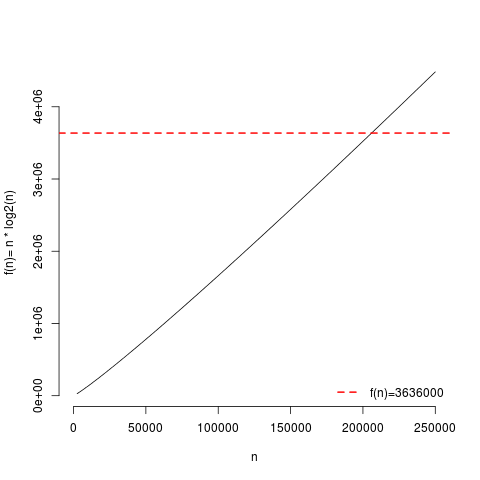
\includegraphics[width=10cm]{exe2}\\

\item $2^n$\\
$2^n=3636000$\\
$n=\log_2{(3636000)}$\\
$n\approx{21}$\\

\pagebreak

\item $2^{2^n}$\\
$n=\log_2{(\log_2{(3636000)})}$\\
$n\approx{4}$

  \end{enumerate}

\item Rearranje a seguinte lista de funções em ordem crescente de taxa de crescimento. Isto é,
se a função $g(n)$ sucede imediatamente a função $f(n)$ na sua lista, então é verdade que $f(n) = O(g(n))$.


\begin{center}

$f1(n) = n^{2.5}$ \\
$f2(n) = \sqrt{2\cdot n}$ \\
$f3(n) = n + 10$ \\
$f4(n) = 10^n$ \\
$f5(n) = 100^n$ \\
$f6(n) = n^2 \cdot \log_2(n)$ \\

\end{center}

\begin{center}

Organizadas em ordem crescente de tempo de execução:

$f2(n) = \sqrt{2\cdot n}$ \\
$f3(n) = n + 10$ \\
$f6(n) = n^2 \cdot \log_2(n)$ \\
$f1(n) = n^{2.5}$ \\
$f4(n) = 10^n$ \\
$f5(n) = 100^n$ \\

\end{center}
\pagebreak

\item Considere o problema de computar o valor de um polinômio em um ponto. 
Dados n coeficientes $a_0 , a_1 , . . . , a_{n-1}$ e um número real $x$, 
queremos computar $\sum\limits_{i=0}^{n-1} a_i \cdot x^i$.
  
  \begin{enumerate}[(a)]
\item Escreva um programa simples com tempo de execução de pior caso $O(n^2)$ para solucionar este problema.

\begin{lstlisting}
#include<stdio.h>
#define MAX 100
float polinomio(int grau, float coef[], float x) {
  int i,j;
  float out=0, pot;

  for(i=0;i<=grau;i++){
    pot=1;
    for(j=1;j<=i;j++){
      pot=pot*x;
    }
    out=out+(coef[i]*(pot));
  }

  return out;
}

int main(void)
{
  int i, grau;
  float coef[MAX],x;

  printf("Entre com o grau do polinomio:");
  scanf("%d",&grau);
  printf("Entre com os coeficientes (do maior para o menor grau):");
  for(i=grau;i>=0;i--){
    scanf("%f",&coef[i]);
  }
  printf("Entre com o valor a ser avaliado:");
  scanf("%f",&x);

  printf("Metodo convencional: f(%f) = %f\n",x,polinomio(grau,coef,x));
  return 0;
}
\end{lstlisting}
\pagebreak

\item Escreva um programa com tempo de execução de pior caso $O(n)$ para solucionar este problema 
usando o método chamado de regra de Horner para reescrever o polinômio:

\begin{lstlisting}
#include<stdio.h>
#define MAX 100
float horner(int grau, float coef[], float x) {
  int i;
  float out=0;
  for(i=grau;i>0;i--) {
    out=(out+coef[i])*x;
  }
  out=out+coef[0];
  return out;
}

int main(void)
{
  int i, grau;
  float coef[MAX],x;
  printf("Entre com o grau do polinomio:");
  scanf("%d",&grau);
  printf("Entre com os coeficientes (do maior para o menor grau):");
  for(i=grau;i>=0;i--){
    scanf("%f",&coef[i]);
  }
  printf("Entre com o valor a ser avaliado:");
  scanf("%f",&x);

  printf("Metodo Horner: f(%f) = %f\n",x,horner(grau,coef,x));
  return 0;
}
\end{lstlisting}
  \end{enumerate}
\pagebreak


\item Seja $A[0...n-1]$ um vetor de $n$ números inteiros distintos dois a dois. Se $i<j$ e $A[i]>A[j]$
então o par $(i,j)$ é chamado uma inversão de A.

  \begin{enumerate}[(a)]
\item Liste as cinco inversões do vetor $A = 2, 3, 8, 6, 1$ .

$S=\{ (3,8) , (3,1) , (8,6) , (8,1) , (6,1) \}$

\item Qual vetor com elementos no conjunto $\{1, 2, . . . , n\}$ tem a maior quantidade de inversões? Quantas são?

O vetor terá a maior quantidade de inversões quando estiver ordenado de forma decrescente. Nesse caso teremos 
$(x_n \geq x_{n-1} \geq x_{n-2} \ldots \geq x_{1})$. De certa forma, o número de inversões corresponde ao quanto 
um vetor está desorganizado, sendo o número de trocas necessarias para organiza-lo.

\item Escreva um programa que determine o número de inversões em qualquer permutação
de n elementos em tempo de execução de pior caso $O(n \cdot \log_2(n))$.

Como o número de inversões é a quantidade de trocas que precisamos realizar para ordenar um vetor, podemos usar
a mesma estratégia de um algoritimo usado para ordenação para processar essa contagem. 
Como nosso objetivo é relizar essa contagem com garantia de um tempo igual a $O(n \cdot \log_2(n))$, podemos tentar
adaptar os algoritimos do mergesort ou heapsort para tal tarefa, aqui adaptamos o mergesort, realizando a contagem
dentro da função intercala e somando todas as contagens dentro da função mergesort.

\begin{lstlisting}
#include <stdio.h>
#define MAX 100

int intercala(int p, int q, int r, int v[MAX])
{
   int i, j, k, w[MAX];
   int inv=0;
   i = p;
   j = q;
   k = 0;
   while (i < q && j < r) {
      if (v[i] < v[j]) {
         w[k] = v[i];
         i++;
      }
      else {
         w[k] = v[j];
         j++;
	 inv = inv + (q - i);
      }
      k++;
   }
   while (i < q) {
      w[k] = v[i];
      i++;
      k++;
   }
   while (j < r) {
      w[k] = v[j];
      j++;
      k++;
   }
   for (i = p; i < r; i++)
      v[i] = w[i-p];
   return inv;
}

/* Recebe um vetor v[p..r-1] e o rearranja em ordem crescente */
int mergesort(int p, int r, int v[MAX]) {
   int q;
   int inv=0;
   if (p < r - 1) {
      q = (p + r) / 2;
      inv  = mergesort(p, q, v);
      inv += mergesort(q, r, v);
      inv += intercala(p, q, r, v);
   }
   return inv;
}

int main(void) {
  int n, i ,vetor[MAX],inv;
  printf("Entre com o numero de elementos:");
  scanf("%d",&n);
  printf("Entre com os elementos:");
  for(i=0;i<n;i++) {
    scanf("%d",&vetor[i]);
  }
  inv=mergesort(0,n,vetor);
  for(i=0;i<n;i++) {
    printf("%d ",vetor[i]);
  }
  printf("\n");
  printf("Existiam %d inversoes\n",inv);
  return 0;
}

\end{lstlisting}


  \end{enumerate}
  
\end{enumerate} %Números

\end{document}
